\documentclass[12pt, a4paper]{article}
\usepackage[headheight = 28pt, margin = 20mm, top = 30mm]{geometry}
\usepackage[brazil]{babel}
\usepackage[utf8]{inputenc}
\usepackage{fancyhdr}
\usepackage{graphicx}
\usepackage{subcaption}
\usepackage{listings}
\usepackage{amsmath}

\lstloadlanguages{Octave}

\pagestyle{fancy}
\fancyhf{}
\lhead{MAC0210\\30/06/2020}
\chead{\textbf{EP2}\\}
\rhead{Cainã Setti Galante 10737115\\Rubens Gomes Neto 9318484}

\begin{document}
\section*{Introdução}
    Para este \textbf{EP} implementamos funções que comprimem e descomprimem imagens
    utilizando os métodos de interpolação bilinear e bicúbica. Com isso testamos
    os métodos em imagens geradas por funções e depois por imagens comuns.

\section*{Implementação}
\subsection*{Compressão, expansão e erro}
    Primeiramente implementamos as funções de compressão e expansão da imagem:
    dependentes do fator de compressão $k$:
    \begin{lstlisting}[language=Octave]
        function compress (originalImg, k)
        function B = expand(A, k)
    \end{lstlisting}
    A função \emph{compress} remove k linhas e/ou colunas entre cada pixel mantido,
    para isso é amostrado um pixel a cada $k+1$ linhas/colunas.\\
    A função \emph{expand} adiciona $k$ linhas e colunas vazias entre cada pixel
    da imagem \textbf{A}, que serão preenchidas pela interpolação escolhida, e
    retorna a nova imagem em \textbf{B}.\\
    \begin{figure}[h]
        \begin{subfigure}{.3\textwidth}
            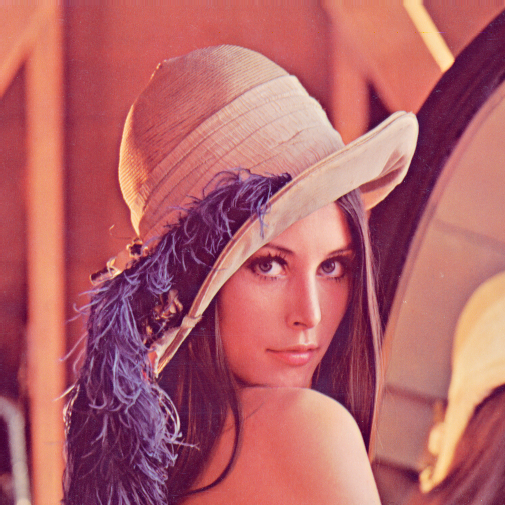
\includegraphics[width=.95\textwidth]{../lenacrop.png}
            \caption{Imagem original}
        \end{subfigure}
        \begin{subfigure}{.3\textwidth}
            
\includegraphics[width=.95\textwidth]{../lenacomp7.png}
            \caption{Imagem comprimida $k=7$}
        \end{subfigure}
        \begin{subfigure}{.3\textwidth}
            
\includegraphics[width=.95\textwidth]{../lenaexp7.png}
            \caption{Imagem expandida $k=7$}
        \end{subfigure}
        \caption{Primeiros processamentos}
    \end{figure}

    Implementamos também uma função que calcula o erro das imagens após o processo
    de compressão e descompressão comparando as diferenças pixel a pixel.
    \begin{lstlisting}[language=Octave]
        function err = calculateError(originalImg, decompressedImg)
    \end{lstlisting}
    Utilizando a seguinte relação:
    \begin{equation*}
        err = \frac{errR + errG + errB}{3},\; \text{onde} \;
        errX = \frac{||origX - decX||_{2}}{||origX||_{2}}, \;
        X \in \{R, G, B\}
    \end{equation*}

\newpage
\subsection*{Bilinear}
    Para a interpolação bilinear implementamos o polinômio aproximador:
    \begin{equation*}
        f(x,y) \approx p_{ij}(x,y) = a_{0} + a_{1}(x - x_{i}) +
        a_{2}(y - y_{j}) + a_{3}(x - x_{i})(y - y_{j})
    \end{equation*}
    Usando os valores dos cantos dos quadrados da imagem original como
    $\{x_i, y_j; x_{i+1}, y_{j+1}\}$. Desta forma calculamos os coeficientes resolvendo o seguinte sistema linear:
    \begin{equation*}
        \begin{bmatrix}
            f(x_i, y_j) \\
            f(x_i, y_{j+1}) \\
            f(x_{i+1}, y_j) \\
            f(x_{i+1}, y_{j+1})
        \end{bmatrix} =
        \begin{bmatrix}
            1 & 0 & 0 & 0 \\
            1 & 0 & h & 0 \\
            1 & h & 0 & 0 \\
            1 & h & h & h^2 \\
        \end{bmatrix}
        \begin{bmatrix}
            a_0 \\
            a_1 \\
            a_2 \\
            a_3 \\
        \end{bmatrix}
    \end{equation*}

\subsection*{Bicúbico}
    Para a interpolação bicúbica utilizamos o seguinte polinômio:
    \begin{equation*}
        f(x,y) \approx p_{ij}(x,y) =
        \begin{bmatrix}
            1 & (x - x_{i}) & (x - x_{i})^2 & (x - x_{i})^3
        \end{bmatrix}
        \begin{bmatrix}
            a_{00} & a_{01} & a_{02} & a_{03} \\
            a_{10} & a_{11} & a_{12} & a_{13} \\
            a_{20} & a_{21} & a_{22} & a_{23} \\
            a_{30} & a_{31} & a_{32} & a_{33} \\
        \end{bmatrix}
        \begin{bmatrix}
            1 \\
            (y - y_{j}) \\
            (y - y_{j})^2 \\
            (y - y_{j})^3
        \end{bmatrix}
    \end{equation*}
    Usando os valores dos cantos dos quadrados da imagem original como
    $\{x_i, y_j; x_{i+1}, y_{j+1}\}$. Para obter os valores $a_{ij}$ resolvemos
    o seguinte sistema:
    \begin{equation*}
        \begin{bmatrix}
            f(x_{i},y_{j})                               & f(x_{i},y_{j+1})                               & \frac{\partial f}{\partial y}(x_{i},y_{j})              & \frac{\partial f}{\partial y}(x_{i},y_{j+1}) \\
            f(x_{i+1},y_{j})                             & f(x_{i+1},y_{j+1})                             & \frac{\partial f}{\partial y}(x_{i+1},y_{j})            & \frac{\partial f}{\partial y}(x_{i+1},y_{j+1}) \\
            \frac{\partial f}{\partial x}(x_{i},y_{j})   & \frac{\partial f}{\partial x}(x_{i},y_{j+1})   & \frac{\partial f}{\partial x \partial y}(x_{i},y_{j})   & \frac{\partial f}{\partial x \partial y}(x_{i},y_{j+1}) \\
            \frac{\partial f}{\partial x}(x_{i+1},y_{j}) & \frac{\partial f}{\partial x}(x_{i+1},y_{j+1}) & \frac{\partial f}{\partial x \partial y}(x_{i+1},y_{j}) & \frac{\partial f}{\partial x \partial y}(x_{i+1},y_{j+1}) \\
        \end{bmatrix} =
        B
        \begin{bmatrix}
            a_{00} & a_{01} & a_{02} & a_{03} \\
            a_{10} & a_{11} & a_{12} & a_{13} \\
            a_{20} & a_{21} & a_{22} & a_{23} \\
            a_{30} & a_{31} & a_{32} & a_{33} \\
        \end{bmatrix}
        B^T
    \end{equation*}
    onde,
    \begin{equation*}
        B = \begin{bmatrix}
            1 & 0 & 0   & 0 \\
            1 & h & h^2 & h^3 \\
            0 & 1 & 0   & 0 \\
            0 & 1 & 2h  & 3h^2 \\
        \end{bmatrix}
    \end{equation*}

\subsection*{Zoológico}
    Para esta parte do EP utilizamos as seguintes funções para gerar as imagens
    de teste:
    \begin{align*}
        f_1(x,y) &= \left(\sin(x), \frac{\sin(y) - \sin(x)}{2}, \sin(x)\right)\\
        f_2(x,y) &= \left(\cos(x), \frac{\sin(y) - \sin(x)}{2}, \sin(y)\right)\\
        f_3(x,y) &= \left(\sin(y), \frac{\sin(y) - \sin(x)}{2}, \begin{cases}
            0, & x \leq \pi\\
            1, & x > \pi
        \end{cases}\right)\\
    \end{align*}
    Geramos imagens de $281\times281$ pixels. Para isso foi feita a transformação
    de pixels de $0$ a $2\pi$ e a saída das funções para $0$ a $1$ para geração
    das imagens. Note que $f_3 \notin C^2$.\\

    \newpage
    As funções geraram as seguintes imagens:
    \begin{figure}[h]
        \begin{subfigure}{.3\textwidth}
            
\includegraphics[width=.95\textwidth]{../fstFun.png}
            \caption{Imagem de $f_1(x,y)$}
        \end{subfigure}
        \begin{subfigure}{.3\textwidth}
            
\includegraphics[width=.95\textwidth]{../secFun.png}
            \caption{Imagem de $f_2(x,y)$}
        \end{subfigure}
        \begin{subfigure}{.3\textwidth}
            
\includegraphics[width=.95\textwidth]{../trdFun.png}
            \caption{Imagem de $f_3(x,y)$}
        \end{subfigure}
        \caption{Imagens originais Zoológico}
    \end{figure}
    As saídas após a compressão e descompressão das imagens com $k=7$ junto a
    seus respectivos erros são:
    \begin{figure}[h]
        \begin{subfigure}{.3\textwidth}
            
\includegraphics[width=.95\textwidth]{../fstFunBL.png}
            \caption{$err = 0.0014335$}
        \end{subfigure}
        \begin{subfigure}{.3\textwidth}
            
\includegraphics[width=.95\textwidth]{../secFunBL.png}
            \caption{$err = 0.0014313$}
        \end{subfigure}
        \begin{subfigure}{.3\textwidth}
            
\includegraphics[width=.95\textwidth]{../trdFunBL.png}
            \caption{$err = 0.024147$}
        \end{subfigure}
        \caption{Imagens descomprimidas utilizando o método bilinear}
    \end{figure}
    \begin{figure}[h!]
        \begin{subfigure}{.3\textwidth}
            
\includegraphics[width=.95\textwidth]{../fstFunBC.png}
            \caption{$err = 0.0043710$}
        \end{subfigure}
        \begin{subfigure}{.3\textwidth}
            
\includegraphics[width=.95\textwidth]{../secFunBC.png}
            \caption{$err = 0.0043806$}
        \end{subfigure}
        \begin{subfigure}{.3\textwidth}
            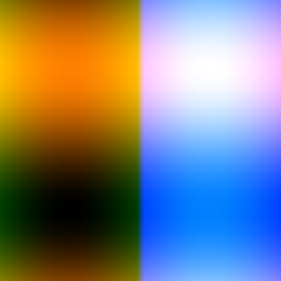
\includegraphics[width=.95\textwidth]{../trdFunBC.png}
            \caption{$err = 0.024140$}
        \end{subfigure}
        \caption{Imagens descomprimidas utilizando o método bicúbico}
    \end{figure}
    Também analisamos a descompressão utilizando um versão preto e branco da imagem
    de $f_3(x,y)$ cujos resultados foram:
    \begin{figure}[h]
        \begin{subfigure}{.3\textwidth}
            
\includegraphics[width=.95\textwidth]{../trdFunBW.png}
            \caption{Imagem original em PB}
        \end{subfigure}
        \begin{subfigure}{.3\textwidth}
            
\includegraphics[width=.95\textwidth]{../trdFunBWBL.png}
            \caption{Bilinear: $err = 0.0070867$}
        \end{subfigure}
        \begin{subfigure}{.3\textwidth}
            
\includegraphics[width=.95\textwidth]{../trdFunBWBC.png}
            \caption{Bicúbico: $err = 0.0070402$}
        \end{subfigure}
        \caption{Imagens preto e branco}
    \end{figure}
    \vspace{2cm}\\
    Após análise da imagens podemos responder que:
    \begin{itemize}
        \item Funciona bem para imagens preto e branco?
        \begin{itemize}
            \item As imagens geradas ficaram bem próximas da original usando tanto
            o método bilinear quanto o bicúbico, com $err < 0.01$ para ambos.
        \end{itemize}
        \item Funciona bem para imagens coloridas?
        \begin{itemize}
            \item As imagens geradas ficaram bem próximas da original usando tanto
            o método bilinear quanto o bicúbico, com $err < 0.01$ para as funções
            $\in C^2$ e $err < 0.1$ para $f_3$.
        \end{itemize}
        \item Funciona bem para todas as funções de classe $C^2$?
        \begin{itemize}
            \item Tivemos erros muito pequenos para todas as funções de $C^2$ e
            as imagens ficaram visualmente muito parecidas.
        \end{itemize}
        \item E para funções que não são de classe $C^2$?
        \begin{itemize}
            \item Tivemos erros muito pequenos para todas as funções que não são
            $C^2$, porém é possível notar que a mudança drástica de cor gerada pela
            discontinuidade de $f_3$ foi "perdida" pois as interpolações suavizam
            a mudança.
        \end{itemize}
        \item Como se comporta o erro?
        \begin{itemize}
            \item Tivemos erros muito pequenos para todas imagens, sempre com $err < 0.1$.
        \end{itemize}
    \end{itemize}

    Podemos também comparar a decompressão direta usando $k=7$ ou três descompressões
    seguidas com $k=1$ obtendo assim:
    \begin{figure}[h!]
        \begin{center}
        \begin{subfigure}{.3\textwidth}
            
\includegraphics[width=.95\textwidth]{../secFunBL111.png}
            \caption{$errOrig = 0.0014338$ \\ $errK7 = 0.000013017$}
        \end{subfigure}
        \begin{subfigure}{.3\textwidth}
            
\includegraphics[width=.95\textwidth]{../secFunBC111.png}
            \caption{$errOrig = 0.0010179$ \\ $errK7 = 0.0042732$}
        \end{subfigure}
        \end{center}
        \caption{Imagens com múltiplas descompressões com $k=1$ \\
                        (a): Bilinear \; (b): Bicúbico}
    \end{figure}
    \newpage

    Podemos observar que no caso bilinear a imagem ficou muito próxima da versão
    com $k=7$, obtendo um erro com o original bem próximo do primeiro caso e com
    um erro da ordem de $10^{-4}$ quando comparado com a primeira descompressão.\\
    Para o caso bicúbico podemos notar que a diferença entre imagens descomprimidas
    foi mais significativa, o que refletiu num erro menor quando comparado com a
    imagem original.

\vspace{1cm}
\subsection*{Selva}
    Para as análises da selva utilizamos a famosa imagem conhecida por \emph{lena}
    comunmente usada em testes e demonstrações de análise de imagem. A imagem original
    tem dimensões $512 \times 512$ pixels porém por razões de redimensionamento
    cortamos a imagem para que tivesse dimensões $505 \times 505$ pixels.

    Assim geramos as seguintes imagens e análises:
    \begin{figure}[h]
        \begin{subfigure}{.3\textwidth}
            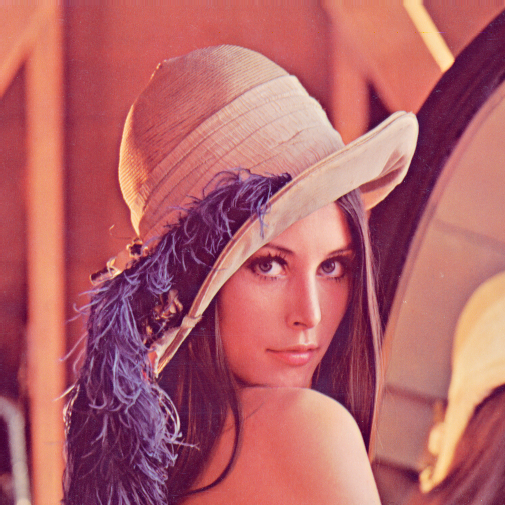
\includegraphics[width=.95\textwidth]{../lenacrop.png}
            \caption{Imagem original\\}
        \end{subfigure}
        \begin{subfigure}{.3\textwidth}
            
\includegraphics[width=.95\textwidth]{../lenaBL7.png}
            \caption{Bilinear $err = 0.032717$}
        \end{subfigure}
        \begin{subfigure}{.3\textwidth}
            
\includegraphics[width=.95\textwidth]{../lenaBC7.png}
            \caption{Bicúbico $err = 0.033258$}
        \end{subfigure}
        \caption{Imagens \emph{lena}, usando $k=7$}
    \end{figure}

    \begin{figure}[h]
        \begin{subfigure}{.3\textwidth}
            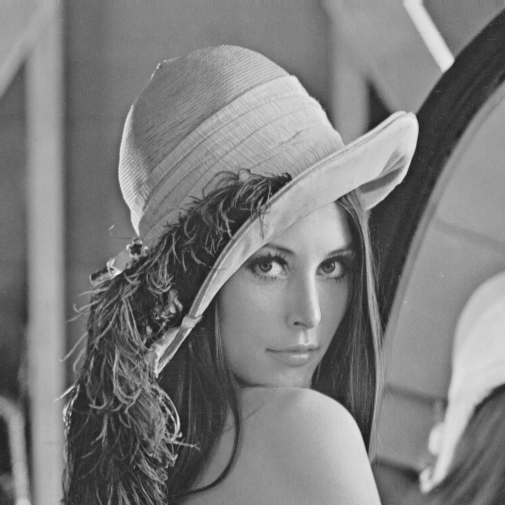
\includegraphics[width=.95\textwidth]{../lenacropBW.png}
            \caption{Imagem original\\}
        \end{subfigure}
        \begin{subfigure}{.3\textwidth}
            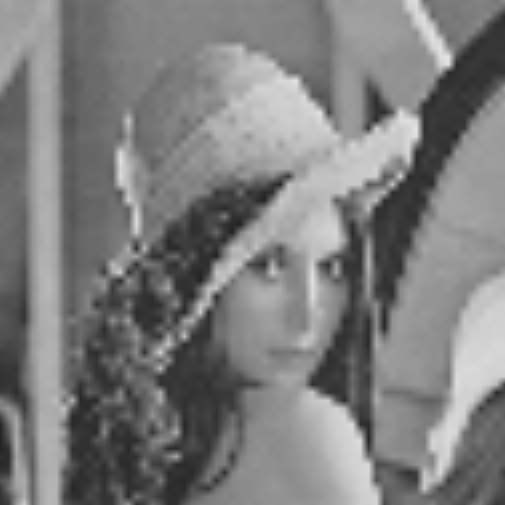
\includegraphics[width=.95\textwidth]{../lenaBWBL7.png}
            \caption{Bilinear $err = 0.031117$}
        \end{subfigure}
        \begin{subfigure}{.3\textwidth}
            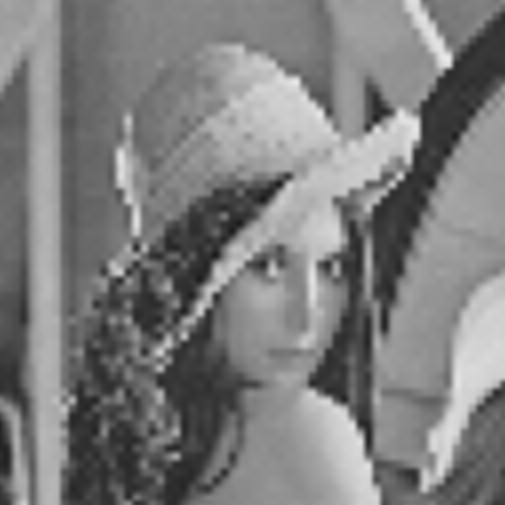
\includegraphics[width=.95\textwidth]{../lenaBWBC7.png}
            \caption{Bicúbico $err = 0.031519$}
        \end{subfigure}
        \caption{Imagens \emph{lena} em PB, usando $k=7$}
    \end{figure}

    \newpage
    \begin{itemize}
        \item Funciona bem para imagens preto e branco?
        \begin{itemize}
            \item As imagens geradas ficaram visualmente diferentes da original
            podendo ser notada uma perda de qualidade da imagem, porém as imagens
            em preto e branco não apresentaram diferença na qualidade quando comparadas
            com suas versões coloridas.
        \end{itemize}
        \item Funciona bem para imagens coloridas?
        \begin{itemize}
            \item Como mencionado acima tivemos perda de qualidade das imagens
            descomprimidas que foram bem mais notáveis do que nos casos do Zoológico,
            com $err \approx 0.03$.
        \end{itemize}
        \item Como se comporta o erro?
        \begin{itemize}
            \item Tivemos erros pequenos para todas imagens, sempre com $err < 0.1$.
        \end{itemize}
    \end{itemize}

    \begin{figure}[h!]
        \begin{center}
        \begin{subfigure}{.3\textwidth}
            
\includegraphics[width=.95\textwidth]{../lenaBL111.png}
            \caption{$errOrig = 0.032759$ \\ $errK7 = 0.0036101$}
        \end{subfigure}
        \begin{subfigure}{.3\textwidth}
            
\includegraphics[width=.95\textwidth]{../lenaBC111.png}
            \caption{$errOrig = 0.033180$ \\ $errK7 = 0.0073432$}
        \end{subfigure}
        \end{center}
        \caption{Imagens com múltiplas descompressões com $k=1$ \\
                        (a): Bilinear \; (b): Bicúbico}
    \end{figure}

    Podemos notar que ambas as imagens geradas com múltiplas descompressões com
    $k = 1$ ficaram bem próximas das geradas com $k = 7$, com $errK7 < 0.1$, e com
    o $errOrig$ muito próximos dos erros da descompressão simples.

\end{document}
